\documentclass{article}

\usepackage{array}       
\usepackage{tabularx}
\usepackage{dcolumn} 
  \newcolumntype{d}[1]{D{.}{.}{#1}}    
\usepackage{booktabs}

\usepackage[table]{xcolor}
\usepackage{pgfplotstable}

\pgfplotstableset{
    color cells/.style={
        col sep=comma,
        string type,
        postproc cell content/.code={%
                \pgfkeysalso{@cell content=\rule{0cm}{2.4ex}\cellcolor{red!##1}\pgfmathtruncatemacro\number{##1}\ifnum\number>50\color{white}\fi##1}%
                },
        columns/x/.style={
            column name={},
            postproc cell content/.code={}
        }
    }
}

\usepgfplotslibrary{colorbrewer}


\begin{document}

% table using D from dcolumn package
\begin{table}

  \centering
  \caption{Table with package dcolumn}
  \begin{tabularx}{\textwidth}{l*{3}{d{-2}}}

  \toprule
            &  \multicolumn{1}{X}{\centering col A} &
\multicolumn{1}{X}{\centering col B} &
\multicolumn{1}{X}{\centering col C} \\
\cmidrule(lr){2-2} \cmidrule(lr){3-3} \cmidrule(lr){4-4}
  \midrule  
       North &      2'228   &   0.300 &  10.6 \\    
       South &        689.2 &   0.8   &   2.6 \\
  \bottomrule

  \end{tabularx}     
\end{table}

\begin{table}\caption{Table as a heatmap}
    \centering
    \pgfplotstabletypeset[color cells]{
    x,a,b,c,d
    a,90,10.5,0,0
    b,0,80,10,10
    c,0,0,95,5
    d,0,10,5,85
    }
\end{table}

\begin{figure}
    \caption{Line plot using colorbrewer}
    \centering
    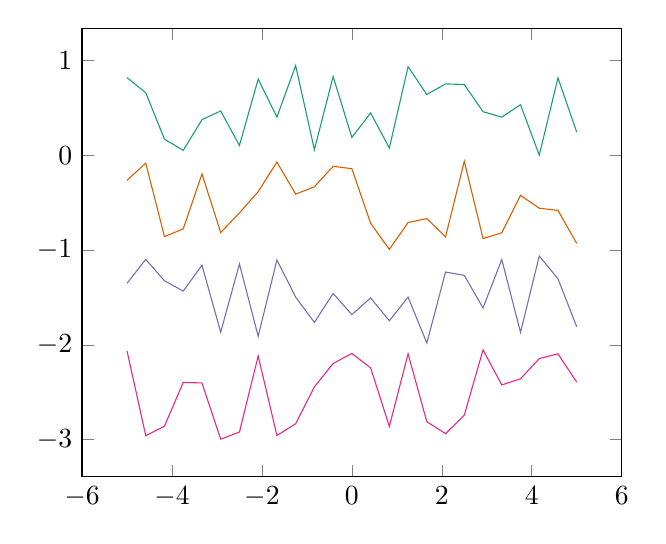
\begin{tikzpicture}
    \begin{axis}[
        cycle list/Dark2,
    ]
    \addplot {rnd};
    \addplot {rnd-1};
    \addplot {rnd-2};
    \addplot {rnd-3};
    
    \end{axis}
    \end{tikzpicture}
\end{figure}

\end{document}